\lab{Animations and 3D Plotting in Matplotlib}{Animations and 3D Plotting in Matplotlib}
\label{lab:lab0}

\objective{Animations and 3D plots are useful in visualizing solutions to ODEs and PDEs found in many dynamics and control problems.
In this lab we explore the functionality contained in the 3D plotting and animation libraries in Matplotlib.}
\labdependencies{}
 
\begin{comment}
\section*{Introduction}
To make animations, we will be using the Matplotlib library.
Matplotlib is a Python library that contains tools for creating plots in multiple dimensions.
The library contains important classes that are needed to create plots.
The most important objects to understand in this lab are figure objects, axes objects, and line objects. 
These three objects can be created using the following code:

\begin{lstlisting}
>>> import matplotlib.pyplot as plt
>>> fig = plt.figure()                  # Create figure object.
>>> ax = fig.add_subplot(111)           # Create axes object.
>>> line2d, = plt.plot([],[])           # Create empty 2D Line object
>>> line3d, = plt.plot([],[],[])        # Create empty 3D line object
\end{lstlisting}

Recall that \li{plt.figure()} creates a \li{matplotlib.figure.Figure} object, which is the window that is displayed when \li{plt.show()} is called.
3D plotting and animation both require explicitly defining the \li{Figure} object, as shown above.
This allows for the object to be updated and modified, as will be explained later in the lab.

\li{Figure} objects contain \li{matplotlib.axes._subplots.AxesSubplot} objects, called \textit{axes}. Axes are spaces to plot on, and are created by the \li{add_subplot()} method of a \li{Figure} object. Figures can have multiple axes. 
%For more information, see [reference Intro to Matplotlib 1 here].

Calling \li{plt.plot()} returns a list of line objects.
For example, supposing \li{x1}, \li{y1}, \li{x2}, and \li{y2} are arrays containing data for two separate curves, then calling \li{plt.plot(x1, y1, x2, y2)} will return a list with two elements.
Each element of the list is a \li{matplotlib.lines.Line2D} object.
If the axes is three-dimensional, then the returned list will contain \li{matplotlib.lines.Line3D} objects.
Because this function call returns a list, if only one line is plotted, adding a trailing comma to the variable name will assign the name to the first element of the returned list.
You can alternatively reference the zero index of the returned list, but using a trailing comma is standard.
\end{comment}

\begin{comment} 
As mentioned in the Introduction to Matplotlib lab in Volume 1, 3D plots and animations are useful in visualizing solutions to ODEs and PDEs found in many dynamics and control problems.
This lab covers basics for 3D plotting, animating 2D plots, and animating 3D trajectories and 3D surfaces. 

In Matplotlib, plots are created using figure objects.
It is possible to create a plot without explicitily instantiating the figure object, but creating an instance separately allows for useful functions to be called on that object. Initializing a figure object is done using the following code:

\begin{lstlisting}
>>> fig = plt.figure()
\end{lstlisting}

3D plotting and animation both require the figure object to be created explicitly. 
\end{comment}
\begin{comment}
\begin{info}
There are different options for plotting in Jupyter Notebook.
In the past we have used \li{\%matplotlib inline}.
For labs with animation we will use \li{\%matplotlib notebook} instead.
This is an interactive regime that allows animations to be displayed without creating a new window.
\end{info}
\end{comment}

\section*{Animation Basics}
The Matplotlib library has a module \li{matplotlib.animation} that has many powerful options
In particular, it contains a class called \li{FuncAnimation} that we will use throughout this lab. 
This class allows us to create animations in a very flexible way.
\li{FuncAnimation} requires a user-defined \textit{update} function that controls the plot for each frame of the animation. 
This grants the user wide flexibility and control of the resulting animation.
The following steps describe the process of creating an animated plot using the \li{FuncAnimation} class:
\begin{enumerate}
\item Create a figure object.
\item Create line objects to be altered dynamically.
\item Choose how to parameterize the frames.
\item Create a function to update line objects.
\item Create a \li{FuncAnimation} object.
\item Display the animation (several methods exist to do so).
\end{enumerate}

\noindent
Let's work through an example of this.
Consider the function
\[
f(x,t) = \frac{1}{1+t}e^{-x^2/(1+t)^2}
\]
modeling the diffusion of heat through a rod.
Suppose that we want to animate how the temperature changes in the segment of a rod for $x\in [-4,4]$ as time evolves from $t=0$ to $t=5$.
In this case, it will be easiest to not precompute the data.
This has a higher risk of making the plot stutter if we just use \li{plt.show()}, but other methods of showing the plot (discussed below) can avoid this issue.

First, we'll set up ranges for $x$ and $t$:
\begin{lstlisting}
import numpy as np

xs = np.linspace(-4, 4, 150)
ts = np.linspace(0, 5, 251)
\end{lstlisting}

Next, we will explicitly create the figure and axis objects, as well a line object that we will update.
Most Matplotlib functions actually return the objects that they manipulate, so this mostly just requires saving the output of the functions we call:
\begin{lstlisting}
from matplotlib import pyplot as plt
from matplotlib.animation import FuncAnimation

# Create a figure and axis object
fig = plt.figure()
ax = fig.add_subplot(1,1,1)
plt.xlim([-2, 2])
plt.ylim([0, 1.1])
\end{lstlisting}
\begin{info}
Many functions for customizing plots (e.g. setting titles, axis ranges, and labels) have different function names when called directly on an axes object.
However, calling from \li{plt} can still be used for these as long as you create subplots one-at-a-time.
More detailed information on the functions available to use with axes objects can be found here: \url{https://matplotlib.org/stable/api/axes\_api.html}.
\end{info}
When we have explicitly defined an axes object, plots are generated by calling the chosen plot function on the axes object (for example, \li{ax.plot(...)}).
The syntax is otherwise identical to calling directly from \li{plt}:
\begin{lstlisting}
# Create an empty line object
# plt.plot actually returns a list of objects; the trailing comma
#   extracts the value from the list
line, = ax.plot([], [], 'r-')
\end{lstlisting}
If we want more lines or also points or scatterplots, we create those here as well.

Next, we need to create the update function.
The \li{FuncAnimation} object will call this function to create each frame of the animation.
The value passed to this function will be a value from our frames list.
Since we aren't precomputing the data we will plot, it will be most convenient to use \li{ts} as the frame values.
In other cases, it can be more useful to use a \li{range()} instead.
So, every time our update function is called, it will be passed the current value of $t$.
We will use the \li{set_data()} method to update the line object we created earlier:
\begin{lstlisting}
def update(t):
    line.set_data(xs, np.exp(- xs**2 / (1+t)**2) / (1+t))
\end{lstlisting}
If we had multiple line objects, we would call \li{.set_data()} on each of them inside of \li{update()}.

Finally, we will create and display the animation:
\begin{lstlisting}
ani = FuncAnimation(fig, update, frames=ts, interval=20)
plt.show()
\end{lstlisting}
The \li{interval} parameter specifies how many milliseconds should be between each frame (as an integer).
Usually we want to choose it so that it takes the animation one second to go from $t=0$ to $t=1$.
If time goes from $t_0$ to $t_f$ and we are using $n_t$ points in our linspace, the right number of milliseconds per frame is given by the following formula:
\[
\text{Interval} \;=
\left\lceil
\frac{1000(t_f-t_0)}{n_t-1}
\right\rceil.
\]
Some additional parameters to \li{FuncAnimation} are given in the table below.

\begin{comment}
These steps will be explained by way of an example.
The arrays \li{x} and \li{y} contain data giving the location of a particle moving in the plane.
To visualize this motion, one could animate the particle as well as display the trajectory that the particle has traveled.
For this animation, two separate \li{Line2D} objects must be created on an axes object.
The first, \li{particle} will be for the position of the particle itself, and the second, \li{traj} will be for the trajectory that the particle has traveled.
Note that these objects are created with empty lists of data.
The update function will be used to dynamically set the data to be plotted in these line objects.

\begin{lstlisting}
>>> import matplotlib.animation as animation
>>> import numpy as np
>>> t = np.linspace(0,2*np.pi,100)
>>> x = np.sin(t)
>>> y = t**2
>>> fig = plt.figure()
>>> ax = fig.add_subplot(111)
>>> ax.set_xlim((-1.1,1.1))
>>> ax.set_ylim((0,40))
>>> particle, = plt.plot([],[], marker='o', color='r')
>>> traj, = plt.plot([],[], color='r', alpha=0.5)
\end{lstlisting}

The update function must be defined a specific way in order to interact properly with the 
\li{matplotlib.animation.FuncAnimation} object.
The update function must accept the current frame index as its first input parameter and it must return a list or tuple of line objects.
The current frame index is used to access the data to be plotted in the current frame. 
Both 2D and 3D line objects have the built-in method \li{.set_data()}.
This function takes in two one-dimensional arrays representing x and y values to plot.
This allows a single line object to display different data for each frame.
Inside the update function, \li{.set_data()} is called on the line objects with the relevant data as inputs.


\begin{lstlisting}
>>> def update(i):
>>>     particle.set_data(x[i],y[i])
>>>     traj.set_data(x[:i+1],y[:i+1])
>>>     return particle,traj
\end{lstlisting}
\end{comment}

\begin{comment}
Three main objects are required for animating plots in Matplotlib.
First, you need to create a figure object as explained above.
Then you need to create a \li{matplotlib.lines.Line2D} or \li{matplotlib.lines.Line3D} object (depending on the dimension of the graph you are animating).
The following code shows one way to initialize a \li{Line2D} object:

\begin{lstlisting}
>>> line, = plt.plot([],[])
\end{lstlisting}

As explained above, \li{plt.plot()} returns a list.
Thus setting the output equal to \li{line,} is equivalent to setting the variable named \li{line} to the first element of the returned list.
Accessing the zero index of the list would yield the equivalent result, but it is conventional to use the trailing comma.

One figure and line objects have been initialized, an update function needs to be defined and a \li{FuncAnimation} object created.
The \li{FuncAnimation} constructor takes in the figure and the update function as inputs.
It calls the update function at each frame of the animation. 

The update function must take the time frame index as its first parameter.
The \li{Line2D} and \li{Line3D} objects have the built in function call \li{set_data()}.
This function takes in 2 1D arrays representing x and y values (or a 2xn array with x and y values). Inside the update function, the \li{set_data()} function is called on the line objects using the frame index to specify the data.
Then the line object is returned, as shown below:

\begin{lstlisting}
>>> def update(i):
>>>     line.set_data(x, y[i])
>>>     return line,
\end{lstlisting}
\end{comment}

\begin{comment}
Next, the \li{FuncAnimation} object is created.
The argument \li{frames} specifies the iterable representing the frame indices.
If \li{frames} is an integer, it is treated as the iterable \li{range(frames)}.
After the \li{FuncAnimation} object is created, \li{plt.show()} displays the animation.

\begin{lstlisting}
>>> ani = FuncAnimation(fig, update, frames=range(100), interval=25)
>>> plt.show()
\end{lstlisting}
\end{comment}

\begin{info}
Using \li{plt.show()} does not work on all platforms (e.g. VSCode).
For alternate methods to show plots, refer to the Saving Animations section below and to the Additional Materials section.
\end{info}

\begin{table}[H]
\label{table:funcanimation-params}
\centering
\begin{tabular}{r|p{0.6\textwidth}}
Parameter & Description\\
\hline
\li{fargs} (tuple) & Additional arguments to pass update function\\
%\li{interval} (float) & Delay between frames in milliseconds\\
\li{repeat} (bool) & Determines whether animation repeats (Default: True.)\\
\li{blit} (bool) & Determines whether blitting is used. (Default: False.) Blitting means that \li{FuncAnimation} will attempt to only update parts of the plot that were actually changed, which may make your animation run faster. If this is enabled, your \li{update} function needs to return a list of all of the line objects that were updated. \\
\end{tabular}
\end{table}

\begin{info}
When using FuncAnimation, it is essential that a reference is kept to the instance of the class.
The animation is advanced by a timer and if a reference is not held for the object, Python will automatically garbage collect and the animation will stop.
\end{info}

\begin{warn}
If you display an animation in a Jupyter notebook using \li{plt.show()}, it will not persist after closing, stopping, and reopening the notebook.
What this means is that when you open the notebook later, there will be a static image in place of your animation.
This is particuarly problematic for turning in an animation to be graded.
Instead of using \li{plt.show()}, save the animation to a file and embed it in your notebook (described below).
\end{warn}

\section*{Saving Animations}
The simplest way to save an animation is to encode it to a \li{.mp4} file, which will allow you to display the video inline inside a Jupyter Notebook, or view it using any video player supporting the chosen filetype.
Unfortunately, Matplotlib does not come with a built-in video encoder.
The \li{matplotlib.animation} module supports several third-party encoders. 
FFmpeg is a lightweight solution that is relatively easy to install:
\begin{itemize}
\item On Linux, run \li{apt-get install ffmpeg} in the terminal, or the equivalent command for your package manager.
\item On Mac, run \li{brew install ffmpeg} in the terminal.
\item On Windows:
	\begin{itemize}
	\item FFmpeg is easiest to install if you have Windows Subsystem for Linux (WSL) installed. In that case, you can run the Linux installation command in your WSL terminal.
	\item Otherwise, you can download it manually from \url{https://github.com/BtbN/FFmpeg-Builds/releases};\footnote{This is one of the sources for the release version endorsed by the FFmpeg website \url{https://www.ffmpeg.org/download.html}.}
	choose one of the versions there marked for Windows.
	If you use this option, you must also manually add its file location to your PATH environment variable.
	\textbf{If this option does not work easily,} it will be easier to just install WSL and use the other option.
	Consult \emph{Getting Started} for instructions on how to do this.
	\end{itemize}
\end{itemize}
To check if you have FFmpeg installed correctly, open your terminal and run the following command:
\begin{lstlisting}
$ ffmpeg
\end{lstlisting}
It should print out a (rather long) help page.

When available, FFmpeg is generally chosen as the default by Matplotlib.
If you get errors, however, you may need to manually specify to Matplotlib to use it:
\begin{lstlisting}
animation.writer = animation.writers['ffmpeg']
\end{lstlisting}
If Matplotlib does not recognize FFmpeg after it is installed, you may also need to restart your Python instance.

Now we proceed to actually saving the animation.
%To prevent the animation from displaying while it is being rendered as video, first use \li{plt.ioff()}.
%This turns off matplotlib's interactive mode until \li{plt.ion()} is called.
After creating the animation object, simply use its \li{.save()} method with the desired filename to render and save the video. 
The following example shows how to do this:
\begin{lstlisting}
plt.ioff()    # Turn off interactive mode to hide rendering animations

# Code to create figure, axes, and update function goes here
# ...
ani = animation.FuncAnimation(fig, update, frames=frames, interval=interval)
ani.save('my_animation.mp4')
\end{lstlisting}
Finally, to display the \li{.mp4} video in a Jupyter Notebook, place the following HTML code in a separate \textbf{markdown} cell (with the filename changed as appropriate):
\begin{lstlisting}
<video src="my_animation.mp4" controls>
\end{lstlisting}

\begin{info}
In Jupyter Notebook, to insert a markdown cell, first insert a new cell, then in the dropdown menu at the top, change the type from Code to Markdown.

If you update the video file, you will need to refresh the markdown cell for the embedded video to update.
To do this, open the markdown cell in text mode again, and then return it to display mode.
% this is probably unhelpful

Remember to push the video files of your animation with the rest of your lab!
\end{info}

\begin{problem}
Use the FuncAnimation class to animate the function $y=\sin(x+3t)$ where $x \in [0,2\pi]$, and $t$ ranges from $0$ to $10$ seconds. 
Save your animation to a file and embed that into the notebook.

Hint: For the \li{frames} argument, use a linspace from 0 to 10.
\end{problem}


\section*{3D Plotting Basics}
3D plotting is very similar to 2D plotting.
The main difference is that a set of 3D axes must be created within the figure object.
A 3D axes object is created using the additional keyword argument \li{projection='3d'}:

\begin{lstlisting}
>>> # Create figure object.
>>> fig = plt.figure()
>>>
>>> # Create 3D axis object using add_subplot().
>>> ax = fig.add_subplot(111, projection='3d')
\end{lstlisting}

3D axes objects can also be created using \li{plt.subplot}; however, many 3D plotting functions only work if you have the axes object, so it is better to use \li{fig.add_subplot}.

\begin{problem}
The orbits for Mercury, Venus, Earth, and Mars are stored in the file \li{orbits.npz}.
The file contains four NumPy arrays: \li{mercury}, \li{venus}, \li{earth}, and \li{mars}.
The first column of each array contains the x-coordinates, the second column contains the y-coordinates, and the third column contians the z-coordinates of each planet, all relative to the Sun, and expressed in AU (astronomical units, the average distance between Earth and the Sun, approximately 150 million kilometers).

Use \li{np.load('orbits.npz')} to load the data for the four planets' orbits.
The \li{.npz} filetype loads as (essentially) a dictionary of arrays; this one has four keys: \li{"mercury"}, \li{"venus"}, \li{"earth"}, and \li{"mars"}.
Create a 3D plot of the orbits along with the starting positions of each planet, and compare your results with Figure \ref{lab0:3dplot}.

Hint: The $z$ range of the data is very narrow. 
Set the $z$ range of the plot manually with \li{ax.set_zlim3d()}.
\end{problem}

\begin{figure}[h]
\centering
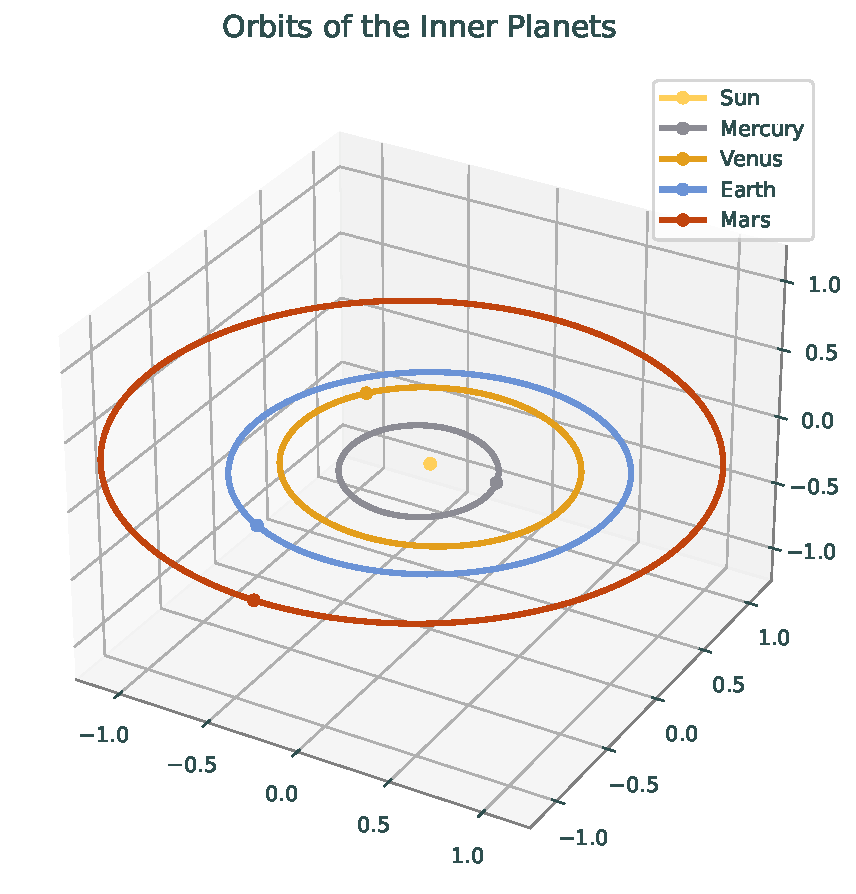
\includegraphics[width=0.7\textwidth]{figures/orbits.pdf}
\caption{The solution to Problem 2.}
\label{lab0:3dplot}
\end{figure}

\subsection*{3D Animations}
The key difference between 2D and 3D animations is that the \li{.set_data()} method does not support setting the \li{z} values.
Instead, use the \li{.set_data_3d()} method, which can be used to update \li{x}, \li{y}, and \li{z} all together.
Note that in order to use this method, the line object must be a 3D line object.
An empty one can be created as follows:
\begin{lstlisting}
line, = ax.plot([], [], [])
\end{lstlisting}

Animation in 3D requires more careful consideration than in the 2D case.
When \li{matplotlib} displays a 3D plot, it does so in an interactive figure that allows the user to change the camera angle and position.
Since 3D rendering is more computationally expensive than 2D rendering, interactive views of 3D animations often have poor framerates and choppy rendering.
This is what calling \li{plt.plot()} attempts to do; instead, it is much better to either render the animation to a file and then embed the file as discussed above (recommended), or to use the HTML5 API to embed it as discussed in Additional Materials (runs faster but often has issues after closing the notebook).

\begin{problem}
\label{prob:animation:planets-anim}
Each row of the arrays in \li{orbits.npz} gives the position of the planets at evenly spaced time points. The arrays correspond to 1400 points in time over a 700 day period (beginning on 2018-5-30).

Create a 3D animation of the planet orbits.
Display lines for the trajectories of the orbits and points for the current positions of the planets at each point in time.
The lines displayed at each frame should only be the part the planet has traveled so far; see Figure \ref{animation:planets-midanimation} for an example of what this should look like.
Embed your animated plot.

Hint: For the \li{frames} argument, use \li{range(1400)}.
The parameter your \li{update()} function will receive will be the \emph{index} of time for the frame, rather than the actual value of time.
This will be useful for slicing arrays.
\end{problem}
\begin{figure}[h]
\centering
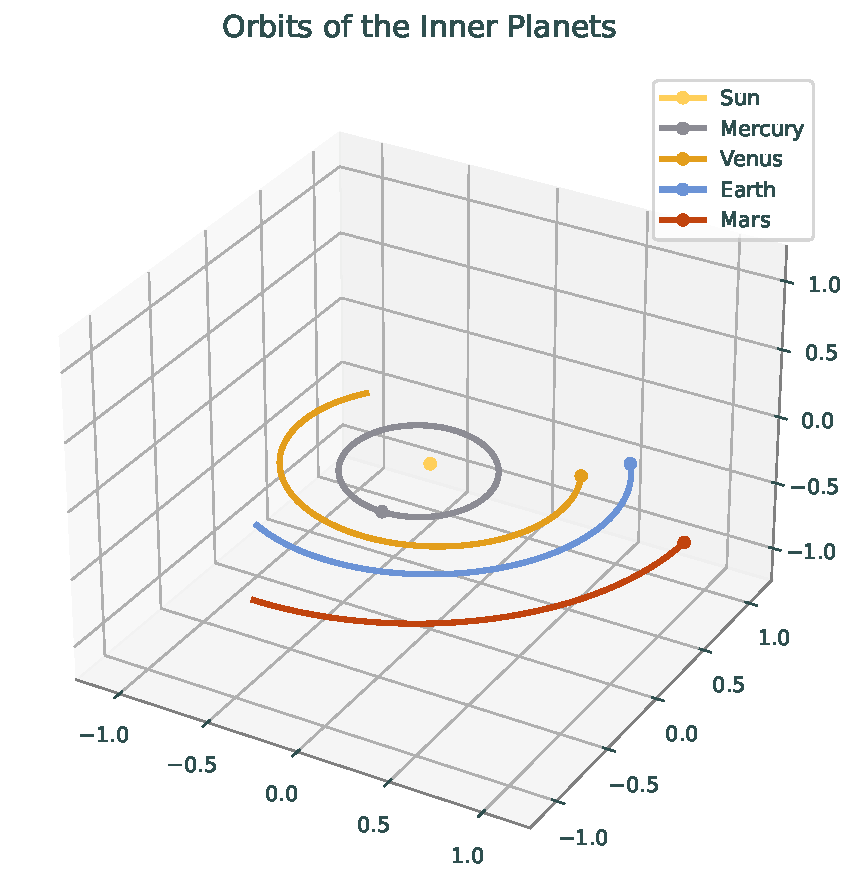
\includegraphics[width=0.7\textwidth]{figures/orbits-midanimation.pdf}
\caption{Example of what your Problem \ref{prob:animation:planets-anim} animation should look like mid-animation.}
\label{animation:planets-midanimation}
\end{figure}

\section*{Surface Plotting}
3D surface plotting is very similar to regular 3D plotting discussed earlier.
With surface plots, however, we must first create a \textit{meshgrid} for X and Y.
The process is identical to how to plot heatmaps and contour plots.

Meshgrids are created using the NumPy command \li{np.meshgrid(x, y)} where \li{x} and \li{y} are 1D arrays representing the x and y coordinates of the grid.
This function creates 2D arrays \li{X} and \li{Y} that combined give cartesian cordinates for every point made from the \li{x} and \li{y} arrays. 
Once a meshgrid is defined, a surface plot is generated by calling \li{ax.plot_surface(X, Y, Z)}, where \li{Z} is a 2D array of height values that is the same shape as \li{X} and \li{Y}. 

\begin{problem}
Make a surface plot of the bivariate normal density function given by

$$f(\mathbf{x})=\frac{1}{\sqrt{\det(2\pi \Sigma)}}\exp{\left[-\frac{1}{2}(\mathbf{x} - \mu)^T \Sigma^{-1} (\mathbf{x} - \mu)\right]}$$

where $\mathbf{x}=[x,y]^T$, $\mu=[0,0]^T$ is the mean vector, and $$\Sigma = \begin{bmatrix} 1 & 3/5 \\ 3/5 & 2 \end{bmatrix}$$ is the covariance matrix. Compare your results with Figure \ref{lab0:surf}.
\end{problem}

\begin{figure}[H]
\centering
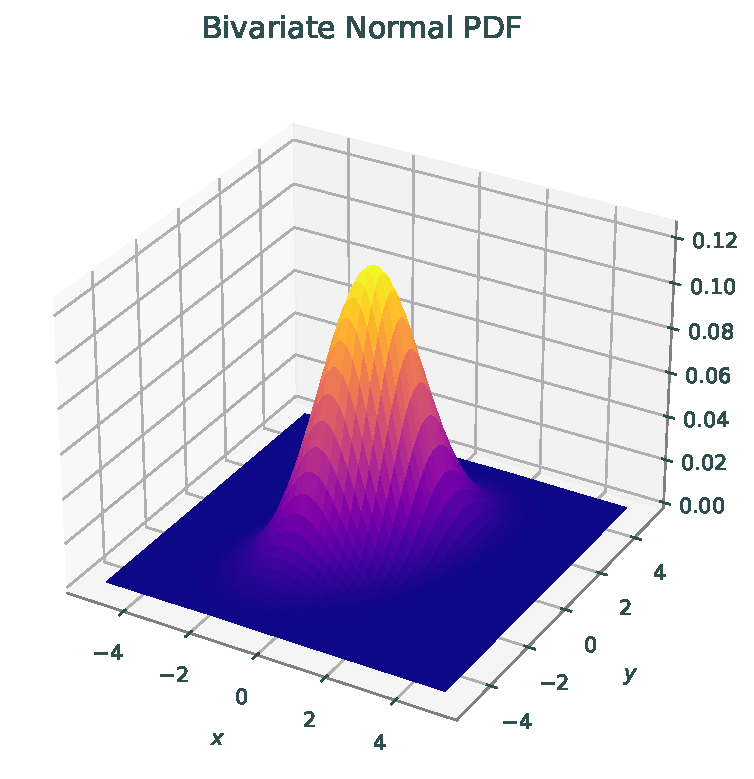
\includegraphics[width=100mm]{figures/normal_density.pdf}
\caption{The solution to Problem 4.}
\label{lab0:surf}
\end{figure}

\subsection*{Surface Animations}
Animating a 3D surface is slightly different from animating a parametric curve in 3D.
The object created by \li{.plot_surface()} does not have a \li{.set_data()} method.
Instead, use \li{ax.clear()} to empty the axes at each frame, followed by a new call to \li{ax.plot_surface()}.
Note that the axis limits must be reset after \li{ax.clear()} is called; otherwise, the limits will change every frame of the animation and it will look rather strange.

\begin{problem}
Use the data in \li{vibration.npz} to produce a surface animation of the solution to the wave equation for an elastic rectangular membrane.
The file contains three NumPy arrays: \li{X}, \li{Y}, \li{Z}.
\li{X} and \li{Y} are meshgrids of shape \li{(300,200)} corresponding to 300 points in the y-direction and 200 points in the x-direction, giving a 2x3 rectangle with one corner at the origin.
\li{Z} is of shape \li{(150,300,200)}, giving the height of the vibrating membrane at each (x,y) point for 150 values of time. 
In the language of partial differential equations, this is the solution to the following initial/boundary value problem:

$$u_{tt} = 6^2(u_{xx}+u_{yy})$$
$$(x,y) \in [0,2]\times[0,3], t \in [0,5]$$
$$u(t,0,y)=u(t,2,y)=u(t,x,0)=u(t,x,3) = 0$$
$$u(0,x,y) = xy(2-x)(3-y)$$
\end{problem}
\begin{warn}
Remember to push your video files with the rest of the lab!
Otherwise, your grader will not be able to view your animations, even if they are correctly embedded in your notebook.

When running \li{git add}, you will need to explicitly specify the video files' filenames the first time you add them: \li{git add animation1.mp4 animation2.mp4 [...]}
\end{warn}

\newpage
\section*{Additional Material}
\subsection*{Directly Embedding Animations}
While saving animations to a file has the advantage that the animation will always persist if the notebook is closed and reopened, it tends to be much slower than directly embedding the animation in the notebook.
Directly embedding can thus be useful in the process of creating an animation by allowing faster experimentation.

After creating an animation, calling \li{plt.show()} will attempt to embed it; however, many systems may struggle to display an animation in this way.
When this is the case, it may be easier to embed the animation using the HTML5 API. 
Jupyter notebooks use HTML to display their contents, so we can leverage this and use HTML5's video capabilities to insert video directly into a notebook.

To embed the video directly into a notebook using HTML5 you must use the \li{IPython.display} module.
This module will be able to interpret an encoded HTML5 video, which can be created by \li{matplotlib.animation}.
This method tends to be much more simple than rendering the animation to an \li{.mp4} file and then embedding that file into a notebook, and it tends to encounter fewer bugs than using \li{plt.show()}.
However, the animation generally does not persist if the notebook is closed and reopened, and this generally still requires FFmpeg to be installed.
Here is a snippet you may reference to embed an animation using \li{IPython.display}
\begin{lstlisting}
# required import statements
from IPython.display import HTML
import matplotlib.pyplot as plt
from matplotlib import animation

# disable interactive mode
plt.ioff()
''' 
Here we would insert whatever code needed to create the animation
such as instantiating the fig object and defining the update function
'''
# create animation
ani = animation.FuncAnimation(fig, update, frames, interval)
# render as html5 and embed
HTML(ani.to_html5_video())
\end{lstlisting}

\begin{warn}
Note that animations that are embedded in the notebook using \li{HTML()} \textbf{\emph{do not always}} persist if the notebook is closed and reopened.
They sometimes do, but are very inconsistent.
While this method can be useful for more quickly testing animations, \textbf{\emph{do not}} use this method for embedding the final animations of your finished lab, as the person grading them will not be able to view your animations.
\end{warn}